Table~\ref{tab:p4-summary-full} extends the summary to all ten runs.

\vspace{1em}
\noindent\begin{minipage}{\linewidth}
\centering
\addtocounter{table}{1}
\label{tab:p4-summary-full}
\begin{tabular*}{\linewidth}{@{\extracolsep{\fill}}lrrrrr}
\toprule
Run & Pass@1 (\%) & Pass@8 (\%) & Gap (\%) & Extr.\ Fail (\%) & $\Delta$ Pass@1 \\
\midrule
Baseline & 9.7 & 24.9 & \textbf{15.2} & 60.3 & --- \\
\midrule
+ A & 12.3 & 33.3 & 21.0 & 34.8 & +2.6 \\
+ B & 10.4 & 26.5 & 16.1 & 53.5 & +0.7 \\
+ A+B & 11.9 & 30.3 & 18.3 & 39.6 & +2.2 \\
\midrule
+ C & 12.9 & 36.2 & 23.4 & 25.3 & +3.2 \\
+ D & 11.8 & 30.4 & 18.7 & 44.5 & +2.0 \\
+ E & 13.8 & 37.2 & 23.4 & 22.7 & +4.1 \\
+ C+D & 12.8 & 37.8 & 24.9 & 22.8 & +3.1 \\
+ C+D+E & 13.1 & \textbf{39.1} & 26.0 & \textbf{15.9} & +3.4 \\
\midrule
Comb.\ All & \textbf{14.6} & 35.6 & 21.0 & 20.0 & +4.9 \\
\bottomrule
\end{tabular*}
\end{minipage}
\vspace{1em}


Number grounding (E) is the strongest individual reward (\pFourSeparateEDeltaPassOne{}pp), surpassing non-degeneracy (C, \pFourSeparateCDeltaPassOne{}pp) and format compliance (A, \pFourSeparateADeltaPassOne{}pp).
The Comb.\ All run achieves the highest Pass@1 at \pFourCombinedAllPassOne\% (\pFourCombinedAllDeltaPassOne{}pp over baseline), while C+D+E achieves the highest Pass@8 (\pFourCombinedCdePassEight\%) and lowest extraction failure rate (\pFourCombinedCdeExtrFail\%).
Figure~\ref{fig:p4-individual-impact} visualizes the Pass@1 ranking and per-problem gains and losses across all configurations.

\vspace{1em}
\noindent\begin{minipage}{\linewidth}
\centering
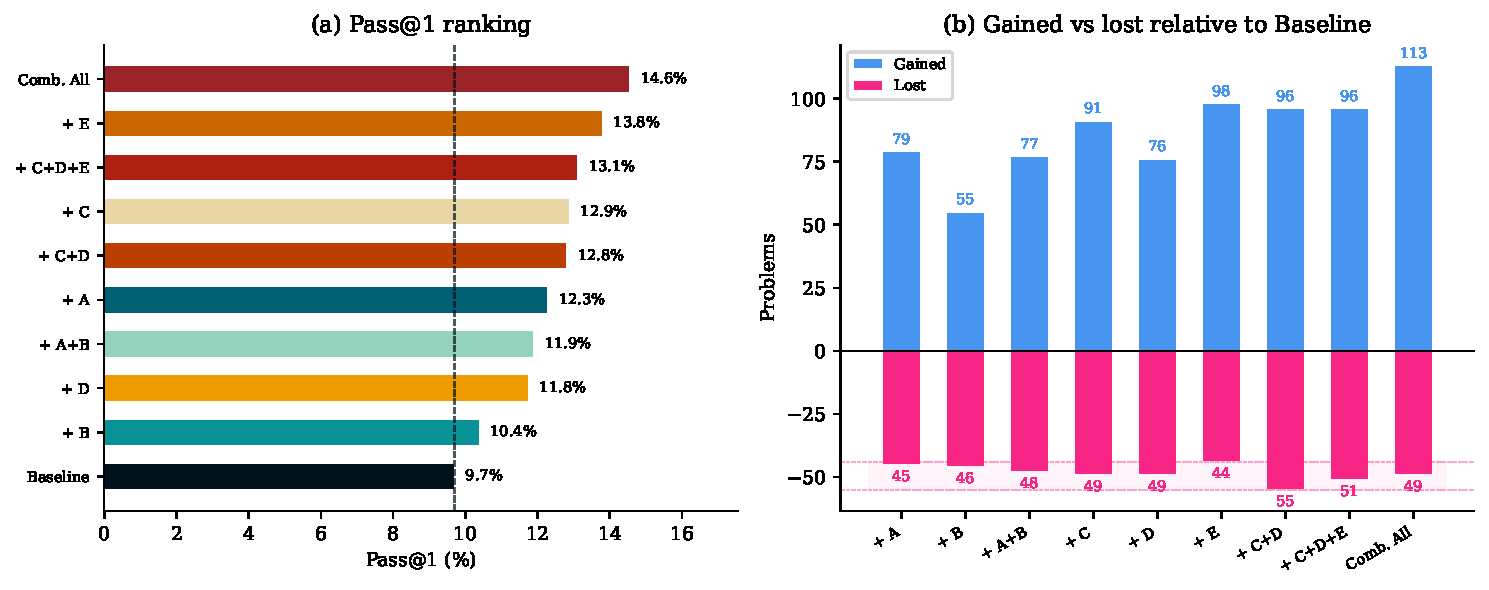
\includegraphics[width=\linewidth]{component/figures/p4/fig2_individual_impact.pdf}
\captionof{figure}{Individual impact of each reward configuration. (a)~Pass@1 ranking; dashed line marks the baseline. (b)~Problems gained (green) and lost (red) vs.\ Baseline; shaded band marks the \pFourLossMin--\pFourLossMax{} loss stability range.}
\label{fig:p4-individual-impact}
\end{minipage}
\vspace{1em}

\vspace{1em}
\noindent\begin{minipage}{\linewidth}
\centering
\addtocounter{table}{1}
\label{tab:p4-gained-lost-full}
\renewcommand{\arraystretch}{0.85}
\begin{tabular*}{\linewidth}{@{\extracolsep{\fill}}lrrr}
\toprule
Run & Gained & Lost & Net \\
\midrule
+ A & 79 & 45 & \textbf{34} \\
+ B & 55 & 46 & 9 \\
+ A+B & 77 & 48 & \textbf{29} \\
\midrule
+ C & 91 & 49 & \textbf{42} \\
+ D & 76 & 49 & \textbf{27} \\
+ E & 98 & 44 & \textbf{54} \\
+ C+D & 96 & 55 & \textbf{41} \\
+ C+D+E & 96 & 51 & \textbf{45} \\
\midrule
Comb.\ All & 113 & 49 & \textbf{64} \\
\bottomrule
\end{tabular*}
\end{minipage}
\vspace{1em}


Reward E gains \pFourSeparateEGained{} problems with the fewest losses of any individual reward (\pFourSeparateELost), yielding the highest individual net (+\pFourSeparateENet).
The Comb.\ All run gains \pFourCombinedAllGained{} problems while losing only \pFourCombinedAllLost{} (net +\pFourCombinedAllNet), more than any other configuration.
The gap between C+D+E's Pass@8 (\pFourCombinedCdePassEight\%) and its Pass@1 (\pFourCombinedCdePassOne\%) is the widest of any configuration (\pFourCombinedCdeGap{}pp), indicating the grounding rewards teach the model to solve many problems but not yet reliably.
The loss count remains stable across all configurations (\pFourLossMin--\pFourLossMax), reinforcing the observation that a fixed population of problems becomes harder under any reward perturbation.
